%!TEX root = ./template-skripsi.tex
%-------------------------------------------------------------------------------
%                            	BAB IV
%               		KESIMPULAN DAN SARAN
%-------------------------------------------------------------------------------

\chapter{UJI COBA DAN HASIL UJI COBA}

\section{Uji Coba}
	Uji coba pada sistem dilakukan terhadap ANGKA responden mahasiswa yang pernah atau sedang menjadi penanggung jawab kelas dan ANGKA dosen dimana di antaranya ANGKA TPjM. Setiap responden akan menguji coba sistem yang telah dikembangkan berdasarkan peran masing-masing responden. Uji coba yang dilakukan menggunakan data yang didapatkan dari hasil sebaran kuesioner \textit{User Acceptance Test}. \textit{User Acceptance Test} bertujuan untuk mengetahui apakah sistem yang dibuat sudah sesuai dengan kebutuhan \textit{user} atau belum. Berikut langkah-langkah pengujian yang akan dilakukan pada sistem informasi Koperasi Mahasiswa Universitas Negeri Jakarta:
\begin{enumerate}
	\item Mahasiswa
	\begin{itemize}
		\item Melakukan \textit{login} menggunakan akun SIAKAD.
		\item Mengunduh RPS.
		\item Membuat pertemuan.
		\item Memvalidasi pertemuan.
		\item Mengisi kehadiran pertemuan.
		\item Memvalidasi presensi kehadiran.
		\item Melihat data presensi kehadiran kelas.
		\item Melihat data tugas dan perhitungan nilai.
		\item Melihat rekap presensi.
		\item Melihat data semester sebelumnya.
	\end{itemize}
	\item Dosen
	\begin{itemize}
		\item Melakukan \textit{login} menggunakan akun SIAKAD.
		\item Mengolah (membuat, menyunting, menghapus) pertemuan.
		\item Memvalidasi pertemuan.
		\item Memvalidasi presensi kehadiran.
		\item Mengisi perizinan mahasiswa.
		\item Melihat data presensi kehadiran kelas.
		\item Mengolah (membuat, menyunting, menghapus) tugas.
		\item Mengunduh dan mengunggah excel nilai.
		\item Memilih penanggung jawab kelas dan penanggung jawab sementara.
		\item Mengunggah dan mengunduh RPS.
		\item Melihat halaman monitoring untuk TPjM.
		\item Melihat data semester sebelumnya.
	\end{itemize}
\end{enumerate}

Pengujian yang dilakukan terdiri dari dua pengujian, yaitu pengujian fungsionalitas dan pengujian kebergunaan atau \textit{usablity}. Pada pengujian fungsional, sistem penilaian yang digunakan berdasarkan pada pilihan: \\

\begin{tabular}{lll}
S& : Setuju\\
TS& : Tidak Setuju\\
\\
\end{tabular}

Pada pengujian kebergunaan (\textit{usability}), sistem penilaian yang digunakan adalah skala likert. Skala likert adalah skala yang terdiri dari serangkaian pernyataan yang menjelaskan sikap responden terhadap objek penelitian. Setiap pernyataan terdapat lima poin dari skala "sangat tidak setuju" hingga "sangat tidak setuju" REF LIKERT.PDF. Setelah didapatkan seluruh data penilaian dari responden, nilai tersebut dikalkulasikan sesuai sistem penilaian berikut:

\begin{itemize}
	\item Nilai Total

		Nilai total adalah jumlah keseluruhan yang didadapat dari tiap pernyataan atau dapat ditulis menjadi: \\
		\(Nilai Total = (jumlah \times skorSS) + (jumlah \times skorS) + (jumlah \times skorC) + (jumlah \times skorTS) + (jumlah \times skorSTS)\)
	\item Persentase Kelayakan

		Persentase kelayakan adalah persentase nilai rata-rata yang didapatkan dengan cara membagi nilai total dengan skor maksimal.  Skor maksimal adalah nilai maksimal skala likert yang dikalikan dengan jumlah pernyataan. Perhitungan tersebut dapat ditulis menjadi: \\
		\(Persentase Kelayakan(\%) = \frac{NilaiTotal}{SkorMaksimal}\times100\)
\end{itemize}

Persentase kelayakan yang sudah didapatkan akan dibandingkan dengan skor pada skala likert untuk menarik kesimpulan akhir dari hasil pengujian. Berikut model skor skala likert:\\

\begin{tabular}{lll}
Sangat Kurang Sesuai& = 0\% - 20\%\\
Kurang Sesuai& = 21\% - 40\%\\
Cukup Sesuai& = 41\% - 60\%\\
Sesuai& = 61\% - 80\%\\
Sangat Sesuai& = 81\% - 100\%\\
\\
\end{tabular}


\section{Hasil Uji Coba}
Berdasarkan hasil uji coba \textit{User Acceptance Test} yang dilakukan terhadap ANGKA responden mahasiswa yang pernah atau sedang menjadi penanggung jawab kelas dan ANGKA dosen dimana di antaranya ANGKA TPjM, diperoleh hasil uji coba sebagai berikut:

\subsection{\textit{Mahasiswa}}
Berikut merupakan daftar pernyataan \textit{User Acceptance Test} pada \textit{Admin}:

\begin{table}[h!]
\begin{center}
\caption{Hasil Uji Fungsionalitas Pada Mahasiswa}
\label{tab:multiplicitybab2}
\begin{tabular} { | >{\centering\arraybackslash}m{1em} | >{\raggedright\arraybackslash}m{22em} | >{\centering\arraybackslash}m{3.7em} | >{\centering\arraybackslash}m{3.7em} | }
	\hline
	\multirow{2}{*}{\textbf{No.}} & \multicolumn{1}{c|}{\multirow{2}{*}{\textbf{Pernyataan}}} & \multicolumn{2}{c|}{\textbf{Jawaban Responden}} \\ 
	\cline{3-4} && \textbf{TS} & \textbf{S}\\
	\hline

	1 & Fitur login berjalan dengan baik. & 0 & 5 \\ \hline
	2 & Fitur daftar kelas dan filter semester berjalan dengan baik. & 0 & 5 \\ \hline
	3 & Fitur download rps berjalan dengan baik. & 0 & 5 \\ \hline
	4 & Fitur mengelola (membuat dan memvalidasi) pertemuan berjalan dengan baik. & 0 & 5 \\ \hline
	5 & Fitur hadir dan validasi presensi berjalan dengan baik. & 0 & 5 \\ \hline
	6 & Fitur tabel presensi berjalan dengan baik. & 0 & 5 \\ \hline
	7 & Fitur tugas dan nilai berjalan dengan baik. & 0 & 5 \\ \hline
	8 & Fitur rekap presensi dan filter semester berjalan dengan baik. & 0 & 5 \\ \hline
	9 & Fitur logout berjalan dengan baik. & 0 & 5 \\ \hline

\end{tabular}
\end{center}
\end{table}

Setelah kuisioner \textit{admin} diberikan kepada responden, kemudian data kuesioner diolah untuk mendapatkan hasil penilaian \textit{user acceptance test}. Adapun hasil penilaian \textit{user acceptance test} tersebut yaitu:

\begin{table}[H]
	\centering
	\caption{Data Hasil Penyebaran Kuesioner \textit{User Acceptance Test} pada \textit{Admin}}
	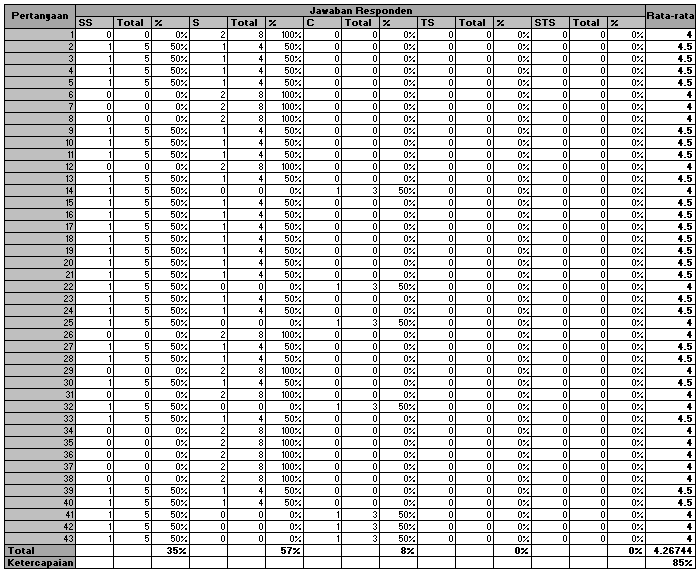
\includegraphics[width=1\textwidth]{gambar/Hasil_Admin}
\end{table}

Dari hasil penilaian pengujian \textit{user acceptance test} dapat diambil kesimpulan yaitu:

\begin{enumerate}
	\item Pengguna sistem yang telah memilih Sangat Tidak Setuju (STS) memiliki persentase 0\%
	\item Pengguna sistem yang telah memilih Tidak Setuju (TS) memiliki persentase 0\%
	\item Pengguna sistem yang telah memilih Cukup (C) memiliki persentase 8\%.
	\item Pengguna sistem yang telah memilih Setuju (S) memiliki persentase 57\%.
	\item Pengguna sistem yang telah memilih Sangat Setuju (SS) memiliki persentase 35\%.
	\item Rata-rata penerimaan \textit{user} adalah 4,27 dari 5 atau sekitar 85\%.
\end{enumerate}

\begin{figure}[H]
	\centering
	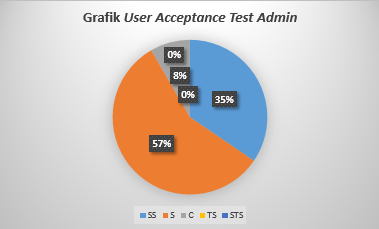
\includegraphics[width=1\textwidth]{gambar/Grafik_Admin}
	\caption{Grafik Hasil Penyebaran Kuesioner \textit{User Acceptance Test} pada \textit{Admin}}
\end{figure}

Berdasarkan hasil pengujian \textit{user acceptance test} yang diujikan kepada 2 responden \textit{admin}, dapat dilihat bahwa secara keseluruhan 35\% menjawab sangat setuju, 57\% menjawab setuju, 8\% menjawab cukup, serta rata-rata penerimaan \textit{user} terhadap kesesuaian sistem dengan kebutuhan adalah 4,27 dari 5 atau sekitar 85\%, oleh karena itu dapat diambil kesimpulan bahwa fitur yang \textit{admin} butuhkan dalam sistem informasi yang dirancang sudah sangat sesuai dengan kebutuhan dan berjalan dengan baik.  

\subsection{\textit{Anggota}}
Berikut merupakan daftar pertanyaan \textit{User Acceptance Test} pada Anggota

\begin{table}[H]
	\centering
	\caption{Daftar Pertanyaan \textit{User Acceptance Test} pada Anggota}
	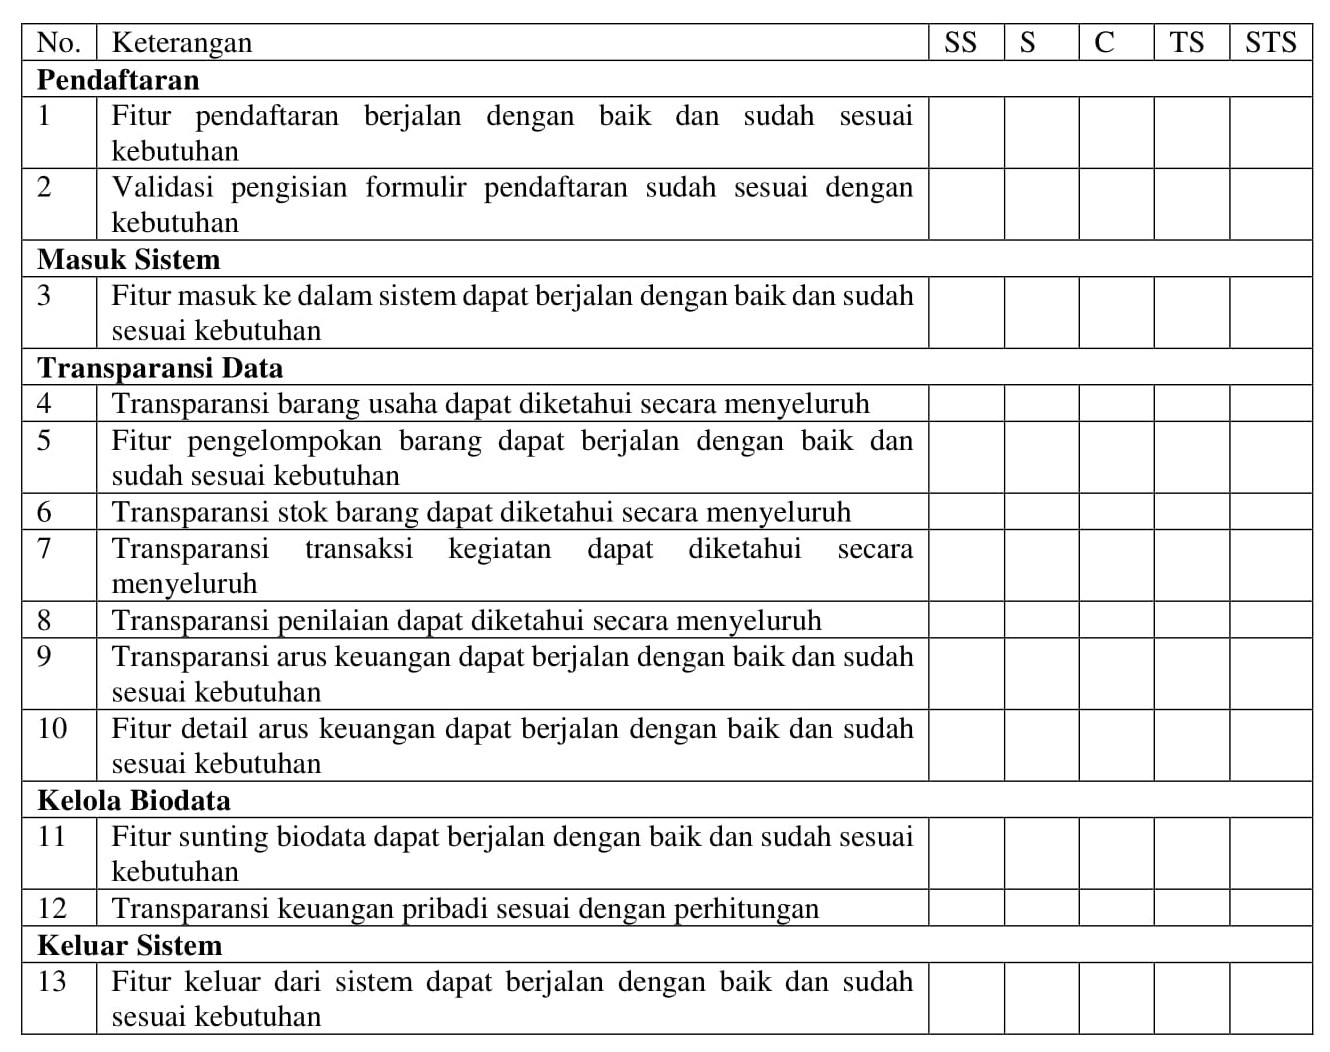
\includegraphics[width=1\textwidth]{gambar/Tabel_Anggota}
\end{table}

Setelah kuisioner anggota diberikan kepada responden, kemudian data kuesioner diolah untuk mendapatkan hasil penilaian \textit{user acceptance test}. Adapun hasil penilaian \textit{user acceptance test} tersebut yaitu:

\begin{table}[H]
	\centering
	\caption{Data Hasil Penyebaran Kuesioner \textit{User Acceptance Test} pada Anggota}
	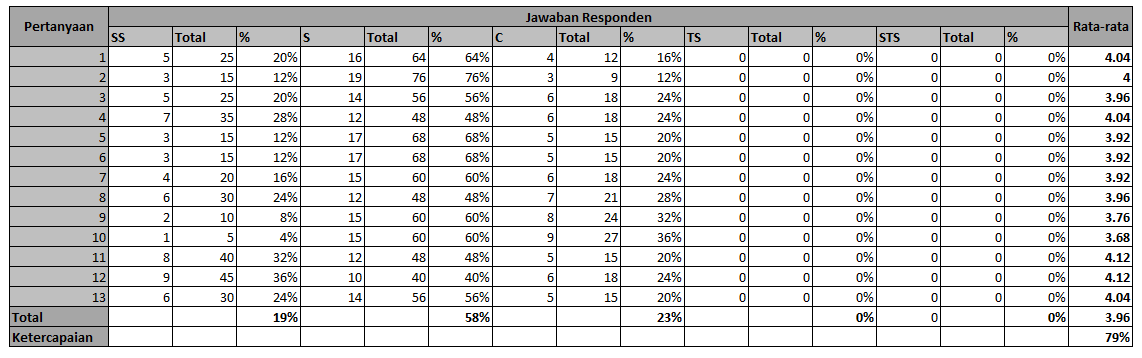
\includegraphics[width=1\textwidth]{gambar/Hasil_Anggota}
\end{table}

Dari hasil pengujian \textit{user acceptance test} dapat diambil kesimpulan yaitu:

\begin{enumerate}
	\item Pengguna sistem yang telah memilih Sangat Tidak Setuju (STS) memiliki persentase 0\%
	\item Pengguna sistem yang telah memilih Tidak Setuju (TS) memiliki persentase 0\%
	\item Pengguna sistem yang telah memilih Cukup (C) memiliki persentase 23\%.
	\item Pengguna sistem yang telah memilih Setuju (S) memiliki persentase 58\%.
	\item Pengguna sistem yang telah memilih Sangat Setuju (SS) memiliki persentase 19\%.
	\item Rata-rata penerimaan \textit{user} adalah 3,96 dari 5 atau sekitar 79\%.
\end{enumerate}

\begin{figure}[H]
	\centering
	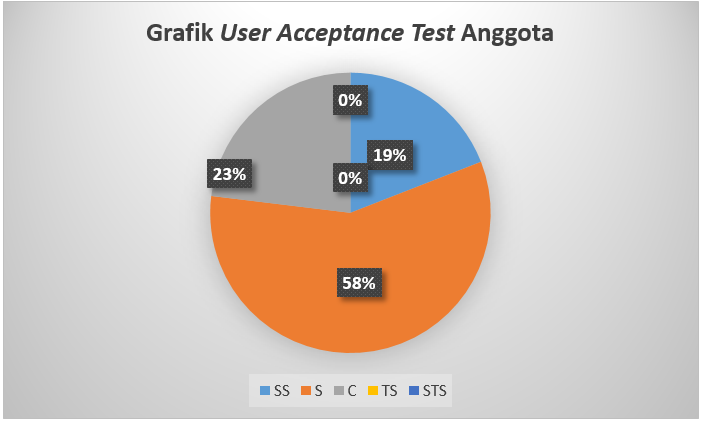
\includegraphics[width=1\textwidth]{gambar/Grafik_Anggota}
	\caption{Grafik Hasil Penyebaran Kuesioner \textit{User Acceptance Test} pada Anggota}
\end{figure}

Berdasarkan hasil pengujian \textit{user acceptance test} yang diujikan kepada 25 responden anggota, dapat dilihat bahwa secara keseluruhan 19\% menjawab sangat setuju, 58\% menjawab setuju, 23\% menjawab cukup, serta rata-rata penerimaan \textit{user} terhadap kesesuaian sistem dengan kebutuhan adalah 3,96 dari 5 atau sekitar 79\%, oleh karena itu dapat diambil kesimpulan bahwa fitur yang anggota butuhkan dalam sistem informasi yang dirancang sudah sesuai dengan kebutuhan dan berjalan dengan baik. 
\\
\\
\\
\\
\\

\subsection{\textit{Pengawas}}
Berikut merupakan daftar pertanyaan \textit{User Acceptance Test} pada Pengawas

\begin{table}[H]
	\centering
	\caption{Daftar Pertanyaan \textit{User Acceptance Test} pada Pengawas}
	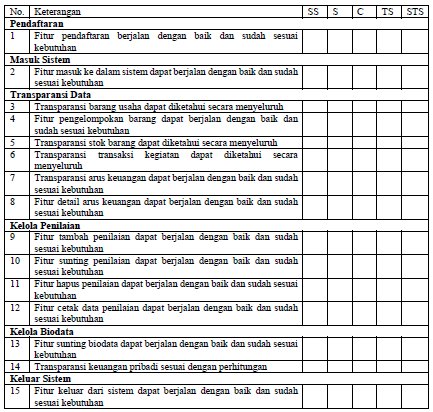
\includegraphics[width=1\textwidth]{gambar/Tabel_Pengawas}
\end{table}

Setelah kuisioner pengawas diberikan kepada responden, kemudian data kuesioner diolah untuk mendapatkan hasil penilaian \textit{user acceptance test}. Adapun hasil penilaian \textit{user acceptance test tersebut} tersebut yaitu:

\begin{table}[H]
	\centering
	\caption{Data Hasil Penyebaran Kuesioner \textit{User Acceptance Test} pada Pengawas}
	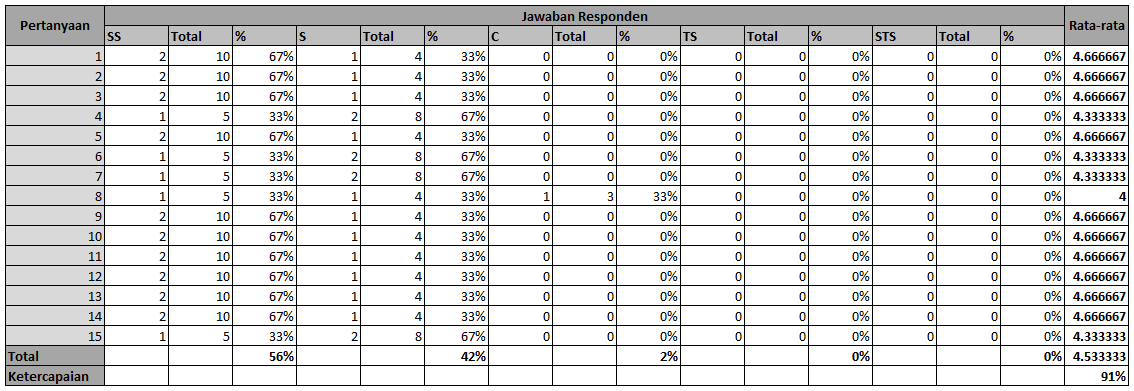
\includegraphics[width=1\textwidth]{gambar/Hasil_Pengawas}
\end{table}

Dari hasil penilaian pengujian \textit{user acceptance test} dapat diambil kesimpulan yaitu:

\begin{enumerate}
	\item Pengguna sistem yang telah memilih Sangat Tidak Setuju (STS) memiliki persentase 0\%
	\item Pengguna sistem yang telah memilih Tidak Setuju (TS) memiliki persentase 0\%
	\item Pengguna sistem yang telah memilih Cukup (C) memiliki persentase 2\%.
	\item Pengguna sistem yang telah memilih Setuju (S) memiliki persentase 42\%.
	\item Pengguna sistem yang telah memilih Sangat Setuju (SS) memiliki persentase 56\%.
	\item Rata-rata penerimaan \textit{user} adalah 4,53 dari 5 atau sekitar 91\%.
\end{enumerate}

\begin{figure}[H]
	\centering
	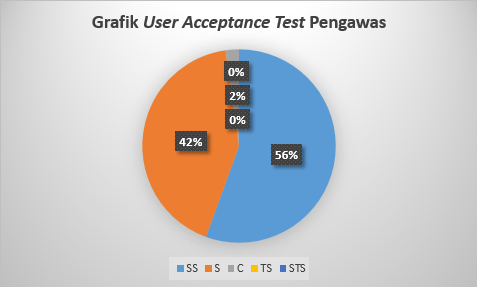
\includegraphics[width=1\textwidth]{gambar/Grafik_Pengawas}
	\caption{Grafik Hasil Penyebaran Kuesioner \textit{User Acceptance Test} pada Pengawas}
\end{figure}

Berdasarkan hasil pengujian \textit{user acceptance test} yang diujikan kepada 3 responden pengawas, dapat dilihat bahwa secara keseluruhan 56\% menjawab sangat setuju, 42\% menjawab setuju, 2\% menjawab cukup, serta rata-rata penerimaan \textit{user} terhadap kesesuaian sistem dengan kebutuhan adalah 4,53 dari 5 atau sekitar 91\%, oleh karena itu dapat diambil kesimpulan bahwa fitur yang pengawas butuhkan dalam sistem informasi yang dirancang sudah sangat sesuai dengan kebutuhan dan berjalan dengan baik. 

% Baris ini digunakan untuk membantu dalam melakukan sitasi
% Karena diapit dengan comment, maka baris ini akan diabaikan
% oleh compiler LaTeX.
\begin{comment}
\bibliography{daftar-pustaka}
\end{comment}